\chapter{結論}
\label{chap:conclusion}
前章まででUIの表層的なデザインは画面内の要素,その優先度,グルーピングで行うことができるのではないかという仮説を立てた.
そして仮説をもとにシステムを実装し,既存UIの再現,ユーザテストを経て本システムの有用性を示すことができた.
本研究により現在では大規模な開発でしか行われていない専門性の高いユーザインタフェースデザインのハードルを下げ,表層のビジュアルデザインに捉われずに,奥深くのデザインに注力する手法を示すことができた.


\section{今後の課題}

要素,優先度,グルーピングからUIを自動生成するシステムの開発に成功したものの,現状の本システムはアプリケーションとしての完成度はとても低く,今後の統合的なシステムとして完成させる必要がある.以下に今後の課題と展望を述べる.
\subsection{要素,優先度,グルーピングの入力UIの検討と開発}
本研究におけるUI自動生成システムではユーザが直接システムを使うことはできず,用紙に要素,優先度,グルーピングを記述してもらい,筆者がシステムが受け付けるコードに変換することで実現している.

今後は要素,優先度,グルーピングを効果的に直感的に入力できるインタフェースの研究開発が必要であり今後の修士課程で,研究を進めていきたい.
\subsection{画面遷移を司るUIの自動生成}
本研究では画面のUIを画面遷移をつかさどるUIと画面のコンテンツを表示するUIの二種類に分類して自動生成をおこなった.
画面遷移を司るUIに関しても法則性を導き出し自動生成を行えるようにしていきたい.これについても今後の修士課程で研究を進めていきたい.
\subsection{配色の自動生成}
実際のUI設計開発では配色はとても重要であり,色によってアプリケーションの見た目や,サービスのブランディングにも大きく影響してくる.

本研究の自動生成システムではiOSアプリでは最もベーシックな白を基調としブルーをアクセントカラーとするデザインが採用されている.ここに関してもサービスのブランディング,ユーザビリティに適した色を提案するシステムを提案したい.これについても今後の修士課程で研究を進めていきたい.

\subsection{スライダーUIによる表層デザインの調整}
本研究における自動生成システムではUIの表層的な見た目は一意に決定されてしまい,自由度がない.プロトタイプやβ版のアプリケーションであれば問題はないが,リリースするプロダクトに本システムを用いるためにはUIをある程度調整できることが不可欠である.これをAdobe Lightroomに習い,スライダーでアプリケーション全ての画面を一括に直感的に変更するシステムも現在研究中であり,本研究のシステムと統合することでより自由度の高く,使いやすいデザインをデザインの専門知識なくとも実現することができる.こちらに関しても修士課程で研究を進めていきたい.

\subsection{統合的なシステムとしての展望}
本研究で開発したUI自動生成システムを基盤とし,前述の課題点を解決するアルゴリズムを開発し,macOS向けのネイティブアプリケーションでの開発を予定している.以下の図\ref{fig:autogen-integrated},図\ref{fig:autogen-integrated2}は現状の統合的なシステムのモックアップである.

\begin{figure}[htbp]
  \begin{minipage}{\hsize}
    \begin{center}
       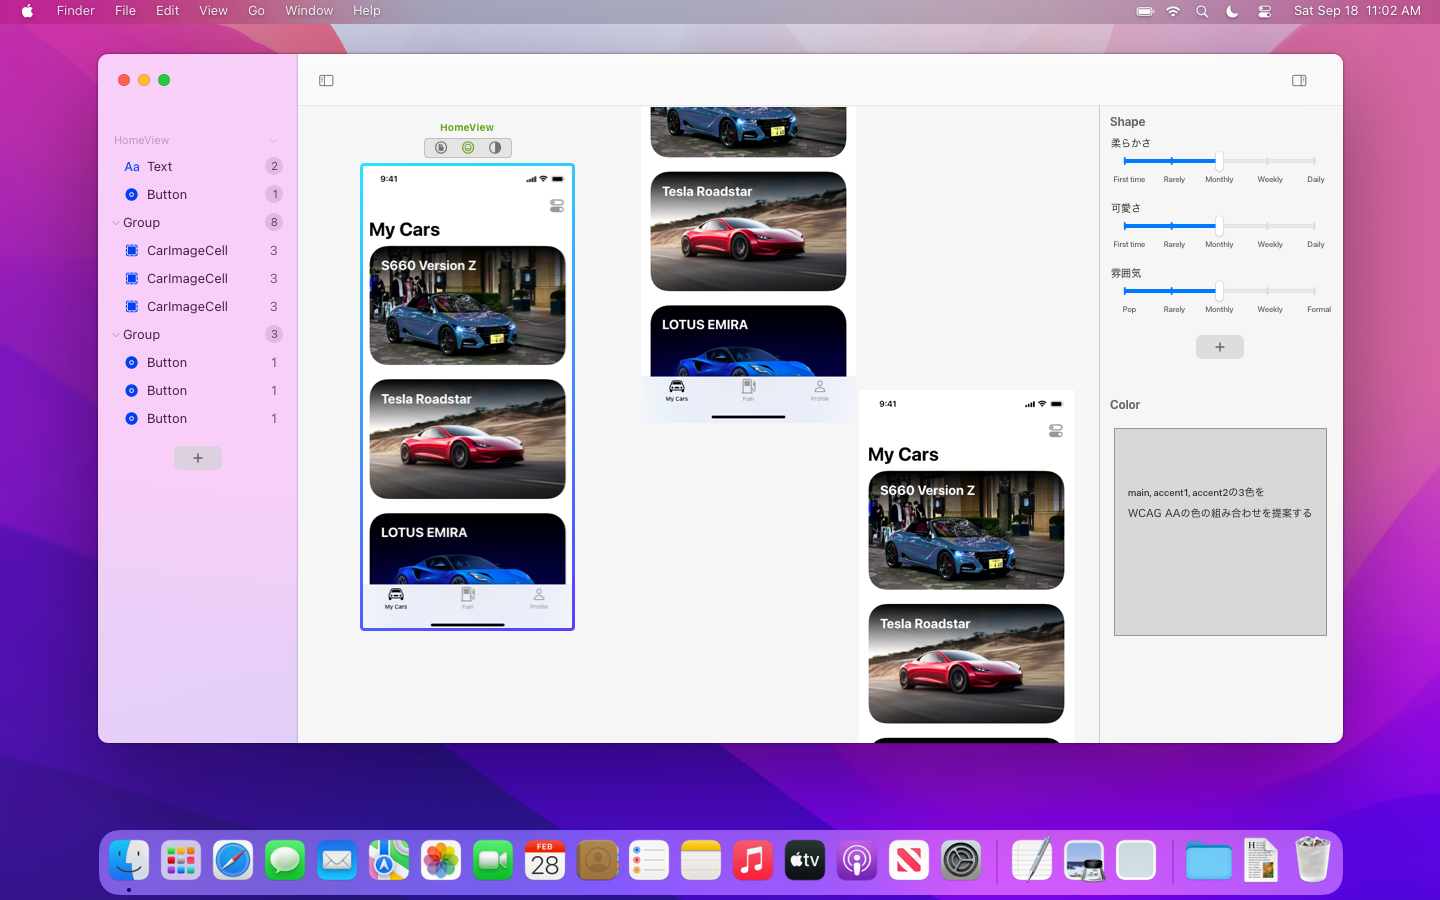
\includegraphics[width=100mm]{img/autogen-integrated.png}
    \end{center}
    \caption{統合デザインシステムのプロトタイプ}
    \label{fig:autogen-integrated}
  \end{minipage}
\end{figure}


\begin{figure}[htbp]
  \begin{minipage}{\hsize}
    \begin{center}
       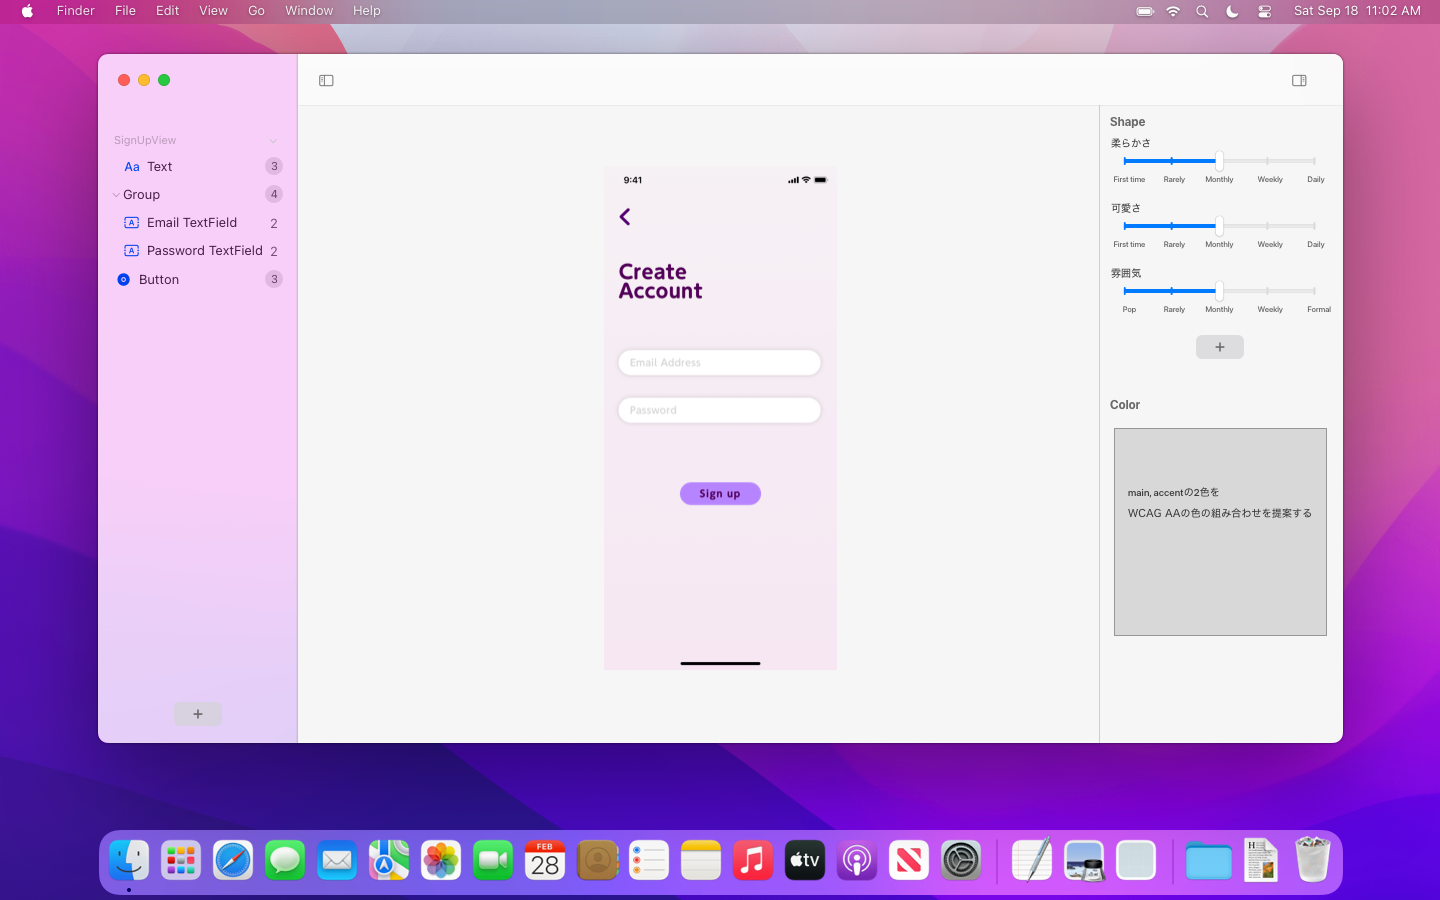
\includegraphics[width=100mm]{img/autogen-integrated2.png}
    \end{center}
    \caption{統合デザインシステムのプロトタイプ2}
    \label{fig:autogen-integrated2}
  \end{minipage}
\end{figure}
